\chapter{2D and Vector Rasterizers}
\label{ch:vector-rasterizers}
\label{ch:sdl-renderer}

\texttt{SDL\_RENDERER} is CNA's simplest renderer, its most exhaustively audited, and the one
whose scope is narrowest by explicit design: a 2D-only rendering path built directly on
SDL3's own 2D texture-blit renderer, with no 3D pipeline, no programmable shader stage, no
depth/stencil buffer, and no multisample antialiasing at all.

It is one of four 2D/vector families in this chapter.  Their common output is a raster image;
the route to that image ranges from SDL texture blits through two CPU rasterizers to an
OpenVG-on-fixed-OpenGL implementation.

\begin{longtable}{p{0.16\textwidth}p{0.27\textwidth}p{0.20\textwidth}p{0.21\textwidth}}
\toprule
Identity & Raster route & 3D result & RT / MRT / query \\
\midrule
\endfirsthead
\toprule
Identity & Raster route & 3D result & RT / MRT / query \\
\midrule
\endhead
\texttt{SDL\_RENDERER} & SDL3 texture-blit API & inherited route rejects & yes / no / no \\
\texttt{SKIA} & Skia raster or Ganesh mode & explicit rejection & yes / no / no \\
\texttt{BLEND2D} & CPU Blend2D, streamed through SDL & inherited route rejects & yes / no / no \\
\texttt{OPENVG} & ShivaVG on fixed-function OpenGL & inherited route rejects & no / no / no \\
\bottomrule
\end{longtable}

\section{Scope, by design}

Every 3D-facing entry point on this renderer --- \texttt{CreateVertexBuffer},
\texttt{DrawColoredPrimitives}, and the rest of the 3D draw dispatch from
Chapter~\ref{ch:backend-architecture} --- throws immediately, with a consistent
\texttt{"SDL\_Renderer does not support 3D"} message. This is not treated as a bug: a
systematic full-suite run confirms exactly thirteen known, expected pre-existing test
failures, every one of them this exact throw, matching the renderer's documented scope
precisely. A custom \cnaclass{Effect} passed to \texttt{SpriteBatch::Begin(effect)} also
throws, for the same underlying reason --- there is no shader stage to run it on.

\subsection{The 2D boundary is at execution, not at every 3D-looking object}

``2D-only'' does not mean that every type normally associated with 3D becomes impossible to
construct.  CNA deliberately distinguishes a renderer-independent description of work from
the first operation that asks this particular renderer to execute that work.  A
\cnaclass{VertexDeclaration}, for example, is only a stride plus a list of
\cnaclass{VertexElement} records; it has no \cnaclass{GraphicsDevice} ownership and no
renderer allocation.  All four of its public constructor shapes therefore work on
\texttt{SDL\_RENDERER}.  The same declaration becomes unsupported only when it is handed to a
real draw call:

\begin{lstlisting}
VertexDeclaration decl(16, {
    VertexElement(0, VertexElementFormat::Vector3,
                  VertexElementUsage::Position, 0),
    VertexElement(12, VertexElementFormat::Color,
                  VertexElementUsage::Color, 0)
});
static const VertexPositionColor vertices[3] = {
    {Vector3::Zero, Color::White}, {Vector3::Zero, Color::White},
    {Vector3::Zero, Color::White}
};

// Construction above is pure data. This execution request throws here:
device.DrawUserPrimitives(PrimitiveType::TriangleList, vertices, 0, 1, decl);
\end{lstlisting}

This is not merely an API-design claim.  The renderer's dedicated regression test constructs
the declaration, confirms that it retains the supplied stride and two elements, then makes the
\texttt{DrawUserPrimitives} call and verifies that the failure happens there rather than while
declaring the layout.  It finally clears and reads back the 2D device successfully, proving
the exception did not leave renderer state unusable.  This boundary lets portable tools and
asset code prepare vertex layouts without a false renderer failure, while still refusing the
first request that would require an SDL renderer 3D pipeline it does not have.

The same split applies to the five stock 3D effects.  \cnaclass{BasicEffect},
\cnaclass{AlphaTestEffect}, \cnaclass{DualTextureEffect}, \cnaclass{EnvironmentMapEffect},
and \cnaclass{SkinnedEffect} can all be constructed, have ordinary properties assigned, and
run \texttt{Apply()} on this renderer.  They are data/configuration objects until a primitive
draw is attempted; that draw still throws.  In particular, the effect test assigns a real
\cnaclass{Texture2D} where applicable but deliberately leaves
\cnaclass{EnvironmentMapEffect}'s \cnaclass{TextureCube} pointer null, separating this
verified lifecycle rule from the still-blocked question of cube-texture construction.

There is a third, easy-to-miss case: \cnaclass{RasterizerState} and
\cnaclass{DepthStencilState} assignments also round-trip as data, but their renderer application
is an intentional no-op.  SDL\_Renderer inherits the interface's no-op
\texttt{ApplyRasterizerState} and \texttt{ApplyDepthStencilState} defaults because neither
state can affect a 2D texture-blit draw.  Code can therefore store and inspect a desired
\texttt{CullMode} or depth-enable bit without an exception; it must not infer that either
state will change pixels.  By contrast, \cnaclass{VertexBuffer} and \cnaclass{IndexBuffer}
constructors immediately call their renderer factories and fail before their own argument
validation runs.  On this renderer even a zero or negative requested count therefore produces
the same explicit ``does not support 3D'' runtime error, rather than an
\texttt{ArgumentOutOfRangeException}.  The ordering is observable and tested, so callers that
need portable validation should validate their input before asking SDL\_Renderer to allocate a
3D buffer.

\subsection{A narrow positive capability among explicit refusals}

Chapter~\ref{ch:backend-architecture}'s \cnaclass{GraphicsCapability} mechanism defaults to
answering \texttt{true} for everything unless a renderer overrides it. Reading
\texttt{SdlRenderer.hpp} directly shows this renderer instead makes one narrow positive claim
and refuses every broader 3D/resource capability:

\begin{lstlisting}
bool SupportsCapability(GraphicsCapability capability) const override
{
    // SDL_ComposeCustomBlendMode represents the standard Additive preset.
    return capability == GraphicsCapability::AdditiveBlending;
}
\end{lstlisting}

Of the current thirteen values, only \texttt{AdditiveBlending} is true. SDL's custom blend mode
can express that preset's independent colour and alpha equations; this does not imply arbitrary
\cnaclass{BlendState} support. \texttt{ThreeD}, complete depth/stencil, standalone stencil,
MSAA, MRT, anisotropy, wireframe, queries, custom effects, volume storage, multistream input and
instancing all return false. The important property is not a blanket answer but an explicit,
auditable boundary: adding the legitimate 2D blend claim did not reopen any 3D promise.

\begin{lstlisting}
if (device.SupportsCapability(GraphicsCapability::ThreeD)) {
    DrawModel(model, world, view, projection);
} else {
    // Reached on SDL_RENDERER (and CANVAS) -- checking first here is strictly better
    // than letting CreateVertexBuffer() or DrawColoredPrimitives() throw
    // "SDL_Renderer does not support 3D" and catching it after the fact.
    DrawFlatPlaceholderSprite();
}
\end{lstlisting}

\section{Recorded SDL Renderer audit and later repairs}
\label{sec:phase70-audit-bugs}

The recorded 65-item technical audit found and fixed fifteen defects across most of the
\cnaclass{SpriteBatch} surface. Its closing document is historical; later repairs described
below supersede parts of that snapshot.

\begin{itemize}
  \item \textbf{SpriteBatch (2 bugs).} \texttt{SDL\_RenderTextureRotated}'s rotation-pivot
        convention did not match XNA's own --- fixed by offsetting the destination
        rectangle. The \texttt{transformMatrix} argument to \texttt{Begin()} was silently
        ignored in its entirety --- fixed via a new path using
        \texttt{SDL\_RenderTextureAffine}, used only for a genuinely non-identity transform
        (Chapter~\ref{ch:spritebatch} covers both in full).
  \item \textbf{SpriteFont (1 bug, shared across every renderer).} The
        \cnaclass{SpriteEffects} flip bug described in Chapter~\ref{ch:spritebatch} ---
        fixed once, in the shared \texttt{SpriteBatch.cpp}, benefiting every renderer at
        once rather than being an SDL\_Renderer-specific fix.
  \item \textbf{BlendState (2 bugs).} Only \texttt{Opaque} and \texttt{Additive} were
        specially handled; every other preset mapped incorrectly. Separately,
        \texttt{SpriteBatch::Begin()} was unconditionally clobbering whatever blend mode had
        already been set, every single call.
  \item \textbf{SamplerState (1 bug).} Four of nine \cnaclass{TextureFilter} values were
        silently downgraded to nearest-neighbor sampling rather than mapping to their real
        \texttt{SDL\_ScaleMode} equivalent.
  \item \textbf{RenderTarget2D (4 bugs).} A shared depth-clear code path crashed outright
        when asked to clear the depth buffer of a render target with
        \texttt{DepthFormat::None} (i.e., no depth buffer at all, which is every render
        target on this 2D-only renderer). A second bug performed an unchecked, unsafe
        downcast between two sibling renderer classes when sampling a render target as an
        ordinary texture --- a genuine memory-safety hazard, not merely a logic error. The
        requested \texttt{DepthFormat} itself is honestly acknowledged as emulated: it is
        silently accepted and echoed back, but no functional depth test exists behind it at
        all on this renderer. A new \texttt{HasRealDepthBuffer()} check was added specifically
        so calling code can ask, rather than assume. The persistent SDL target texture also
        makes shared \cnaclass{RenderTargetUsage} behavior unusually direct: Discard is
        black-cleared on bind, while Preserve and Platform retain color. The strong usage test
        proves the first two with pixels, but its ``every bind'' wording omits CNA's divergence
        from FNA: a redundant bind clears again here, while FNA returns early.
  \item \textbf{Present timing (1 fixed runtime bug, 1 remaining construction asymmetry).}
        Runtime \texttt{PresentInterval::Two} used to collapse silently to
        \texttt{One}. \texttt{SetSwapInterval()} now sends the exact value~2 to
        \texttt{SDL\_SetRenderVSync()} and falls back to~1 if the driver rejects it. The
        constructor still uses \texttt{swapInterval > 0 ? 1 : 0}, despite SDL3 supporting
        integer intervals there too. This usually stays hidden because \cnaclass{Game}
        constructs with the default~1 and later requests arrive through the repaired reset
        path; direct \cnaclass{GraphicsDevice} construction with \texttt{Two} still loses the
        distinction. ASCII wraps this same renderer and inherits both behaviors.
  \item \textbf{Presentation formats (stored, not selected).} Neither the constructor nor a
        later reset receives the requested backbuffer/depth format: the factory passes only
        window, logical-presentation, and swap-interval fields. SDL chooses the renderer's
        window output, while every CNA-created SDL texture is RGBA32 and no depth/stencil
        attachment exists. Fullscreen is different: shared device code still makes SDL's
        window transition request before the renderer's empty format hook.
        The dedicated fullscreen test therefore proves stored state, no throw, and continued
        pixels --- not display acceptance under Xvfb. ASCII inherits this complete split too.
  \item \textbf{Disposed-resource guards (3 bugs).} A missing disposed-texture check inside
        the internal sprite-push path; a missing equivalent check in
        \texttt{SetRenderTargets}; and a dangling renderer pointer left behind after
        \texttt{RenderTarget2D::Dispose()}.
  \item \textbf{OcclusionQuery (1 bug).} Construction previously succeeded silently even with
        a null renderer --- now throws, consistent with the 2D-only-renderer pattern of
        failing loudly at construction rather than producing a query object that can never
        do anything.
\end{itemize}

\section{One blocked sampler decision, and one resource gap that later closed}

One renderer-local architecture decision remains open; the former resource-construction item no
longer does:

\begin{description}
  \item[\texttt{TextureAddressMode::Wrap} / \texttt{Mirror} via \texttt{SpriteBatch}.]
        \texttt{SDL\_RenderTexture}'s own \texttt{srcrect} handling has exactly one fixed,
        clamp-like behavior at the edges. SDL3 does expose
        \texttt{SDL\_SetRenderTextureAddressMode}, but it only affects
        \texttt{SDL\_RenderGeometry} --- an entirely different draw call than the one this
        renderer's \texttt{Draw()} actually issues. Three concrete options were identified and
        none chosen: throw unconditionally whenever \texttt{Wrap} / \texttt{Mirror} is
        requested, rewrite \texttt{Draw()} onto \texttt{SDL\_RenderGeometry} project-wide, or
        a hybrid that only throws when the source rectangle actually exceeds the texture's
        bounds (the common case where it does not would keep working, coincidentally, under
        the existing clamp-like behavior).
  \item[\texttt{Texture3D} / \texttt{TextureCube}: former silent-resource gap, now closed.]
        \cnaclass{Texture3D} now consults the false \texttt{Texture3D} capability and throws
        \cnaclass{NotSupportedException} during construction. A plain \cnaclass{TextureCube}
        may still exist as a renderer-independent description with no native resource, but its
        public \texttt{SetData}/\texttt{GetData} paths detect that absence and throw instead of
        accepting a write or fabricating a transparent-black face. Shared read/write contract
        fixtures pin both outcomes on this renderer. The old 94-test blast-radius note explains
        why the first proposed blanket-construction change was deferred; it is not the current
        observable contract.
\end{description}

\subsection{What ``clamp-like by coincidence'' means in pixels}

The blocked \texttt{TextureAddressMode::Wrap} / \texttt{Mirror} decision above is easy to read
as an abstract API gap; a concrete pixel case makes it precise instead. Take a $2\times1$
texture, texel~0 red and texel~1 blue, and draw it with a source rectangle \emph{twice} the
texture's own width --- source texel range $[0,4]$ against a 2-texel-wide texture, the classic
XNA scrolling-background tiling technique, which FNA's real \cnaclass{SpriteBatch} never clamps
\texttt{sourceRectangle} to the texture's own bounds to prevent:

\begin{lstlisting}
Texture2D redBlue(getGraphicsDeviceProperty(), 2, 1);
const Color pixels[2] = {Color::Red, Color::Blue};
redBlue.SetData(pixels, 2);

Rectangle oversizedSource(0, 0, 4, 1); // spans texel [0,4] on a 2-texel-wide texture
spriteBatch_->Begin(SpriteSortMode::Deferred, BlendState::Opaque, &pointClamp, nullptr, nullptr);
spriteBatch_->Draw(redBlue, destRect, oversizedSource, Color::White);
spriteBatch_->End();
\end{lstlisting}

Reading back the destination pixel corresponding to source position $1.25$ (three-quarters of
the way into the oversized range, past the real 2-texel-wide texture entirely) is where the
``clamp-like, by coincidence'' finding becomes a concrete, checkable number rather than a
qualitative claim: with \texttt{PointClamp} requested, the correct XNA answer is
\textbf{blue} --- clamped to the texture's last real texel --- and \texttt{SDL\_RenderTexture}'s
one fixed edge behavior genuinely produces exactly that, with zero production code written to
make it happen. Requesting \texttt{PointWrap} at the identical source position is where the
still-open gap becomes equally concrete: the XNA-correct answer for a wrapped read at position
$1.25$ is \textbf{red} (wrapping back around to texel~0), but this renderer's \texttt{Draw()}
produces \textbf{blue} again --- the same fixed clamp-like behavior applies regardless of which
\cnaclass{TextureAddressMode} was actually requested, since (per the finding above)
\texttt{SDL\_RenderTexture} has no address-mode parameter reachable from this specific draw
path at all. A game relying on horizontally-scrolling tiled backgrounds --- a common enough
technique that this is not a hypothetical edge case --- gets the wrong pixel on this renderer
today, silently, with no exception and no visual artifact obviously identifiable as ``wrong''
unless you already know to look for texel~0 failing to reappear at the wrap boundary.

\section{Native and emulated behavior}

Beyond the \texttt{DepthFormat} case above, \texttt{TextureAddressMode::Clamp} is flagged as
working ``by coincidence'' --- it matches \texttt{SDL\_RenderTexture}'s own fixed
out-of-bounds behavior, not because any real sampler-state value is being honored.
\texttt{MultiSampleCount} is accepted and ignored, always reporting zero. Fullscreen
toggling round-trips correctly at the API level, but the audit is explicit that genuine
OS-level fullscreen state cannot actually be verified inside this project's own headless
\texttt{Xvfb} test environment. \texttt{ClearOptions::DepthBuffer} / \texttt{Stencil} expose
a shared-routing distinction from the rest of this chapter's 3D methods. The renderer's six
direct combination hooks do call \texttt{ThrowNo3D}, but public
\cnaclass{GraphicsDevice}\texttt{.Clear} first sees \texttt{SupportsDepthStencil()==false} and masks
both bits away. A depth/stencil-only request is therefore an FNA-faithful silent no-op; adding
\texttt{Target} still clears colour. The two SDL-specific tests that expect public throws
predate that mask and are stale; they do not establish that the direct hooks are reachable.
Chapter~\ref{ch:graphicsdevice} and \S\ref{sec:backend-clear-matrix} separate the shared and
renderer layers in full. Five real, multi-frame compatibility samples --- a 2D
demo, a bouncing-sprite physics scene, a keyboard-driven sprite, a two-glyph
\cnaclass{SpriteFont} test, and an animated spritesheet --- are registered as genuine
\texttt{ctest} entries rather than left as manual verification, giving this renderer
end-to-end coverage beyond its unit-level pixel tests.

Viewport and scissor expose a more subtle 2D-state boundary. There is no
\texttt{SetViewport()} override, so a custom public viewport changes stored state and
\cnaclass{Viewport}'s own projection mathematics but never remaps an SDL sprite. Scissor
\emph{does} reach SDL: a positive \texttt{ScissorRectangle} installs a renderer clip, and a
non-positive size disables it. However, the rasterizer-state hook is also absent. The clip is
consequently active solely because
the rectangle is non-empty, even when
\texttt{RasterizerState.ScissorTestEnable == false}. The existing rasterizer construction test
cannot detect this: it verifies no-throw assignment and getter round trip, then clears one
pixel, but never sets a scissor rectangle or asks whether drawing outside it survives. This is
the precise distinction the inherited fourteen-product audit matrix in
\S\ref{sec:backend-viewport-scissor-matrix} preserves.

\section{Reading the feature matrix for this renderer}

The repository's feature-matrix document is a dated planning snapshot, not a live test census.
Its historical custom-\cnaclass{Effect} refusal remains accurate, but its two blocked rows do
not: only \texttt{Wrap}/\texttt{Mirror} still needs the renderer-architecture decision described
above; cube/volume silent success was closed by the shared resource-contract repairs. Current
claims in this chapter therefore come from the registered renderer tests and pinned source, not
from the snapshot's old pass total or status count.

\section{Xvfb screenshot evidence}

Screenshots credited to CNA's \texttt{SOFTWARE} renderer (Chapter~\ref{ch:graphicsdevice}) need
no display server. \texttt{SDL\_RENDERER}, by contrast, creates an SDL3 window and submits
\texttt{SDL\_RenderTexture} calls through an OpenGL context. The retained campaign therefore
used \texttt{Xvfb} with Mesa's \texttt{llvmpipe}. Earlier feasibility notes had identified this
route but left it untested; CNA's \texttt{CNA\_TEST\_DISPLAY} cache variable already permits a
virtual display such as \texttt{:99} in place of the default \texttt{:0}.

Building this renderer (\texttt{cmake -B build-sdlrenderer -DCNA\_GRAPHICS\_RENDERER=SDL\_RENDERER})
and running the screenshot demo under \texttt{xvfb-run} exercised the display and capture path.
The demo reuses the same scene as the golden-image regression test
\texttt{modules/renderers/easygl/examples/\allowbreak{}easygl\_spritebatch\_rotation\_golden\_test.cpp},
also used in Chapter~\ref{ch:spritebatch}: a
$100\times100$ \cnaclass{Texture2D} whose top-left $20\times20$ block is red and the remainder
blue, drawn through \cnaclass{SpriteBatch} rotated $90$ degrees ($\texttt{MathHelper::PiOver2}$)
around \texttt{origin}~$(100,100)$ --- the source's own bottom-right corner --- then captured
with the same \texttt{SaveBackBufferScreenshotEXT} helper the \texttt{SOFTWARE} renderer
screenshots use:

\begin{lstlisting}
xvfb-run -a --server-args="-screen 0 1024x768x24" \
    env -u WAYLAND_DISPLAY ./build-sdlrenderer/cna_xvfb_screenshot_demo
\end{lstlisting}

\begin{figure}[h]
\centering
\begin{figurealt}{SDL Renderer screenshot of a SpriteBatch rotation fixture. A red marker rotated ninety degrees around the source bottom-right origin lands at the destination rectangle's top-right corner.}
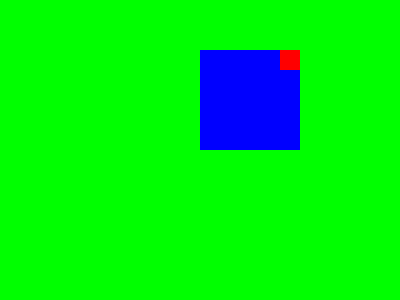
\includegraphics[width=0.5\textwidth]{images/ch17-spritebatch-rotation-sdlrenderer.png}
\end{figurealt}
\caption{Output of the rotate-around-origin \cnaclass{SpriteBatch} scene rendered by
\texttt{SDL\_RENDERER} under \texttt{Xvfb}, without a physical GPU or desktop. The red marker
lands in the destination rectangle's top-right corner, the expected result of a $90$-degree
rotation about the source's bottom-right corner.}
\label{fig:ch17-spritebatch-rotation}
\end{figure}

The marker position matches the geometric derivation used by the golden test
(Chapter~\ref{ch:spritebatch}). The retained artifact closes the screenshot-infrastructure
feasibility item for a renderer that requires a virtual display.

\section{Pixel readback and presentation mode}

The pixel fixtures share one prerequisite, documented in their source comments:

\begin{quote}
\emph{Requires \texttt{PresentationMode::NativeBackBuffer}:
\texttt{SDL\_RenderReadPixels} operates in physical output coordinates, while this renderer's
default presentation mode (\texttt{FixedHeightDynamicWidth}) does not map logical pixels 1:1
to physical ones.}
\end{quote}

\texttt{GetBackBufferData()} delegates to \texttt{SDL\_RenderReadPixels}, which reads physical
output coordinates. \texttt{FixedHeightDynamicWidth} may letterbox logical output, so a logical
coordinate does not necessarily name the same physical pixel. \texttt{NativeBackBuffer} makes
the two sizes equal. The fixtures select it explicitly; without that precondition, a plausible
coordinate check can sample the wrong pixel.

\subsection{Animated sprite-sheet frame selection}

\texttt{modules/renderers/sdl-renderer/examples/\allowbreak{}sdlrenderer\_sample\_animated\_spritesheet\_test.cpp},
the fifth entry in a five-sample compatibility suite, exercises a different route from the
single-frame checks above. These samples use multiple \texttt{Update()} calls. The fixture covers
the \texttt{SpriteBatch::Draw} \texttt{sourceRectangle} parameter, re-selected every
\texttt{Update()} call to animate through a spritesheet. The deterministic sheet is an
$8\times4$ texture, left $4\times4$ solid red (frame~0), right $4\times4$ solid green
(frame~1), with a fixed per-\texttt{Update()} frame-index increment instead of
elapsed-time-based timing, so the outcome never depends on wall-clock frame speed:

\begin{lstlisting}
void Update(GameTime&) override
{
    if (done_) return;
    ++frameCounter_;
    ++updatesRun_;
}

void Draw(const GameTime&) override
{
    // ...
    const int frameIndex = frameCounter_ % 2;
    const Rectangle srcRect(frameIndex * kFrameSize, 0, kFrameSize, kFrameSize);
    const Rectangle destRect(2, 2, kFrameSize, kFrameSize);

    sb_->Begin();
    sb_->Draw(*sheet_, destRect, srcRect, Color::White);
    sb_->End();
    // ...
}
\end{lstlisting}

After exactly three \texttt{Update()} calls, \texttt{frameCounter\_ \% 2} evaluates to
\texttt{1}, so the animation should have settled on the green frame. The test then reads the
rendered pixel instead of checking the frame-index arithmetic alone:

\begin{lstlisting}
Color px(0, 0, 0, 0);
Rectangle region(3, 3, 1, 1);
dev.GetBackBufferData(&region, &px, 0, 1);
check(px.getRProperty() <= 15 && px.getGProperty() >= 240 && px.getBProperty() <= 15,
      "frame 1 (green) reached the rendered output");
\end{lstlisting}

Without \texttt{PresentationMode::NativeBackBuffer}, the frame index can be correct while the
pixel check samples a scaled or letterboxed coordinate. That failure would concern fixture
setup, not animation.

\section{SKIA: a bounded contract written down before expansion}

\texttt{SKIA} is the only renderer whose dependency is neither a system library nor fetched by
the project.  Configuration requires a separately built Skia artifact through
\texttt{CNA\_SKIA\_ROOT} and \texttt{CNA\_SKIA\_BUILD\_DIR}; absence is fatal.

\texttt{CNA\_SKIA\_MODE} selects raster or Ganesh inside the family.  It is not a second public
renderer identity.  Both modes retain the same CNA contract and must be named separately only
when their execution evidence differs.

The implementation has a deliberately bounded 2D surface.  It owns CPU-raster targets and
explicitly rejects 3D, MRT, MSAA, and occlusion queries.  Optional SkSL extensions widen
specific shader-like operations without turning the renderer into a general
\cnaclass{ShaderEffect} route.  The companion capability matrix explains each refusal rather
than relying on a default-true switch; this is one of the strongest capability-documentation
patterns in the repository.

\section{BLEND2D: CPU vectors presented as an SDL texture}

\texttt{BLEND2D} fetches pinned Blend2D and AsmJit revisions unless root overrides are supplied.
It rasterizes on the CPU, uploads the resulting pixels to a streaming SDL texture, and uses SDL
only for the final presentation edge.

The family implements 2D targets.  It has no MRT, query, or 3D path; inherited extended draws
reach the explicit refusal.  Per-channel color-write masks are not natively expressible in its
current compositor, a useful example of a state property that can exist in the public object
without a portable 2D mapping.

The evidence should separate CPU raster output from streaming-texture presentation.  Direct
buffer inspection can prove shape and blend math, while only a real SDL present/readback path
can prove pitch, upload format, and final channel order.

\section{OPENVG: a vector API on a historical GL substrate}

\texttt{OPENVG} uses ShivaVG, pinned to its only upstream commit, plus a local leak patch, a
synthesized configuration header, a GL type shim, and GLU.  The resulting OpenVG~1.1 path runs
over fixed-function OpenGL and needs a real compatible context.

Its capability policy returns false for all 13 flags.  That is conservative but internally
coherent: the renderer supplies its 2D drawing surface without promising the broader GPU
features those flags describe.  It has no render-target factory, MRT, queries, shaders, or 3D;
effect-aware draws inherit the common route and reject.

\section{Four ways to prove a 2D renderer}

For SDL Renderer, observe the actual SDL target and presentation mode.  For Skia, name raster
or Ganesh and test the bounded SkSL path separately.  For Blend2D, compare the CPU pixels before
and after SDL upload.  For OpenVG, capture the GL implementation and context profile alongside
the vector result.  A single screenshot can look identical across all four while exercising
four materially different ownership and delivery paths.
